\documentclass{scrreprt}
\usepackage[utf8]{inputenc}
\usepackage[T1]{fontenc}
\usepackage{lmodern}
\usepackage[francais]{babel, varioref}
\usepackage{graphicx}
\usepackage{listings}

\usepackage{xspace}
\usepackage{amssymb}
\usepackage{calc}
\usepackage{listingsutf8}
\usepackage{color}
\usepackage{xcolor}

%%%%%%%%%%%%%%%%%%%%%
\usepackage{url}
\usepackage[top=2.1cm,bottom=2.2cm,left=2cm,right=2cm]{geometry}
\usepackage[final]{pdfpages}
%%%%%%%%%%%%%%%%%%%%%%%%%%%

%%%%%%%%%%% Pour sommaire cliquable %%%%%%%%%%
\usepackage{hyperref} % Créer des liens et des signets
\hypersetup{
colorlinks=true, %colorise les liens
breaklinks=true, %permet le retour à la ligne dans les liens trop longs
urlcolor= blue, %couleur des hyperliens
linkcolor= black, %couleur des liens internes
citecolor=black,  %couleur des références
}
%%%%%%%%%%%%%%%%%%%%%%%%%%%%%%%%%%%%%%%%%%%%


\newcommand\TODO[1]{\textcolor{red}{\textbf{#1}}}

%pour la coloration du code

\definecolor{colFond}{rgb}{0.8,0.9,0.9}
\definecolor{hellgelb}{rgb}{1,1,0.8}
\definecolor{colKeys}{rgb}{0,0,1}
\definecolor{colIdentifier}{rgb}{0,0,0}
\definecolor{colComments}{rgb}{0,0.5,0}
\definecolor{colString}{rgb}{0.62,0.12,0.94}

\lstset{
  language=c++,
  float=hbp,
  basicstyle=\ttfamily\small,
  identifierstyle=\color{colIdentifier},
  keywordstyle=\bf \color{colKeys},
  stringstyle=\color{colString},
  commentstyle=\color{colComments},
  columns=flexible,
  tabsize=3,
  frame=single,
  frame=shadowbox,
  rulesepcolor=\color[gray]{0.5},
  extendedchars=true,
  showspaces=false,
  showstringspaces=false,
  numbers=left,
  firstnumber=1,
  numberstyle=\tiny,
  breaklines=true,
  backgroundcolor=\color{hellgelb},
  captionpos=b,
}

\usepackage{templateINSA}
\initINSA

\title{PAO Optitrack-drone}

\author{Alexandre \bsc{Brehmer}\\ Christophe \bsc{Cluizel}}
\renewcommand\soustitre{Rapport de projet}
\renewcommand\infoBig{Projet d'Approfondissement et d'Ouverture}
\renewcommand\infoSmall{ASI4 2014-2015}

\begin{document}
 \titleINSA{15}{images/page_couverture.png}{0}{-30}{225}{\url{http://www.lexus-int.com/amazinginmotion/}{\textcolor{white}{}}}

\tableofcontents

\chapter{Introduction}
\TODO{}

\newpage
\chapter{Présentation des systèmes Optitrack et ARDrone}

    % ============= Système Optitrack =============
    \section{Système Optitrack}
        Le système Optitrack est un système permettant de détecter des marqueurs infrarouges grâce à un nombre plus ou moins important de caméras infrarouges. Ce système est composé de caméras (au minimum 3) reliées à un hub usb lui-même relié à un ordinateur et d'un logiciel de traitement des données nommés Motive. \\

        Ce logiciel permet de calibrer les caméras ensembles, de fixer l'origine du repère par rapport aux caméras, de créer des rigidbodies à partir de marqueurs infrarouges et d'obtenir la position des différents marqueurs dans l'espace (et donc des rigidbodies). \\

        Le logiciel Motive peut fonctionner de façon autonome, mais également en tant que serveur couplé à une autre application. En effet, une application cliente peut se connecter à lui afin de récupérer les informations des marqueurs infrarouges et les utiliser de manière extérieure au logiciel Motive. L'architecture suit celle d'une architecture client-serveur.


    % ============= Système ARDrone =============
    \section{Système ARDrone}
       L'ARDrone est un quadricoptère de la marque Parrot. Il est équipé d'un ordinateur ARM 9 cadencé à 468 MHz, d'une RAM de 128 Mo, d'une connectivité Wi-Fi et d'une autonomie de 12 minutes. Il embarque également un accéléromètre 3 axes et un gyroscope 3 axes lui permettant de se stabiliser.\\
Il est par ailleurs équipé deux caméras, un frontal et une ventral aidant à sa stabilisation.\\
 Bien qu'il embarque un ordinateur, le drone n'est pas nativement programmable, il n'est que commandable en orientation, altitude et inclinaison.

\newpage
\chapter{Objectifs du PAO}
\TODO{}

\newpage
\chapter{Calendrier et répartition des tâches}

%============= Calendrier ===================
\section{Calendrier}

	Nous travaillons sur la base d'objectifs d'une durée de 2 semaines maximum. Cela permet de faire un point toutes les 2 semaines avec le responsable du PAO, M. Guerrero, afin d'orienter les objectifs suivants.

% ============= Répartition des tâches ===================
\section{Répartition des tâches}
	Les phases du PAO ont été réalisées en peer-programming, c'est-à-dire en binôme sur une même tache. Cela était indispensable pour la mise en place d'un environnement de développement viable. En effet, il a fallu rechercher et prendre en main les différents outils pour avoir une base stable et commune, puis tester les différentes implémentations en situation réelle avec le drone.

	\begin{figure}
	\hspace{-1cm}
	\begin{tabular}{|@{}l@{}l}
		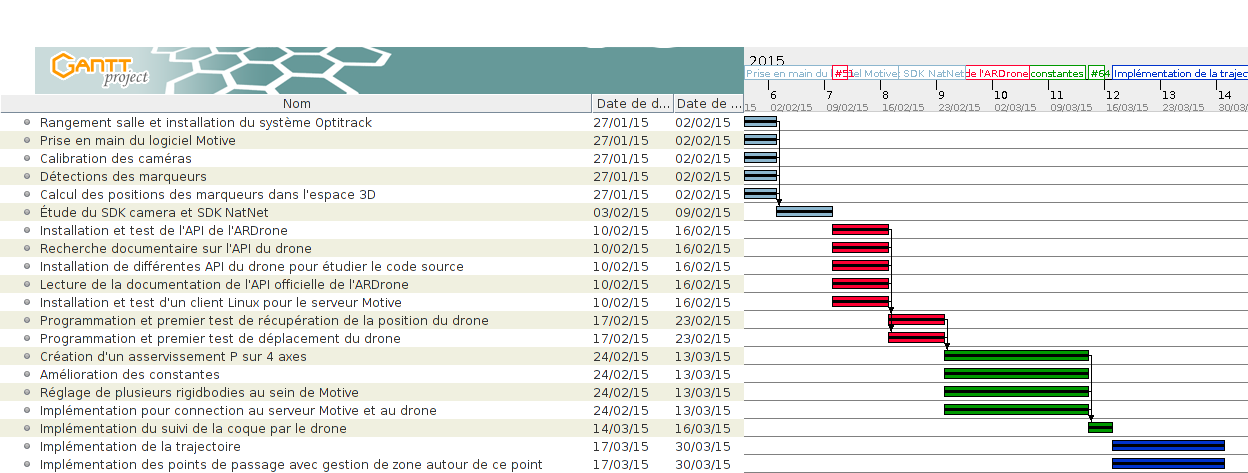
\includegraphics[width=24cm,angle=90]{images/calendrier.png}
	% &
	% 	\includegraphics[width=24cm,angle=90]{images/repartitionCharge.png}
	 \end{tabular}
	 \caption{Planning}
	 \end{figure}

\newpage
\chapter{Suivi de projet}
Les comptes-rendus retracent les objectifs, les réalisations, ainsi que le temps estimé pour réaliser ces objectifs.

%============= Compte rendu à la date du 08/02 ==============
\section{Compte rendu à la date du 08/02}
L'objectif de ces premières semaines étaient de prendre en main le système Optitrack. Pour cela, plusieurs sous objectifs étaient à atteindre: ranger la ``salle drone'', installer les caméras, prendre en main le logiciel Motive, calibrer les caméras, détecter les marqueurs et obtenir leur position, étudier le SDK camera et le SDK NatNet.

%---------------- Alexandre Brehmer -------------------------
\subsection{Alexandre Brehmer}
Tâches effectuées:
\begin{itemize}
	\item pouet \\
\end{itemize}

Temps estimé:????????h.


%---------------- Christophe Cluizel -------------------------
\subsection{Christophe Cluizel}

Tâches effectuées:
\begin{itemize}
	\item rangement de la salle et optimisation de l'espace
	\item installation du système Optitrack
	\item prise en main du logiciel Motive
	\item calibration des caméras
	\item détection des marqueurs
	\item calcul des positions des marqueurs dans l'espace 3D
	\item étude du SDK camera et SDK NatNet \\
\end{itemize}

Temps estimé: 19h.

\newpage
\chapter{Tutoriel}
\section{Prise en main de l'ARDrone}
L'ARDrone est un quadricoptère grand public contrôlable en wifi avec un smartphone. Dans le cadre du PAO, nous avons pour objectif de le faire voler en asservissant sa position dans l'espace grâce au système OptiTrack.
\subsection{Test de vol}
Avant de s'aventurer à commander le drone depuis un PC, nous avons désiré savoir s'il était fonctionnel. Pour cela nous avons téléchargé l'application fournie par Parrot (la marque du drone).\\
\url{https://itunes.apple.com/fr/app/free-flight/id373065271?mt=8}\\
\url{https://play.google.com/store/apps/details?id=com.parrot.freeflight&hl=fr}\\
Une fois la batterie installée à bord, le drone s'allume tout seul et diffuse un réseau wifi dont le SSID ressemble à \textit{ardrone\_XXXX}. Il faut alors connecter le smartphone au réseau wifi du drone et lancer l'application téléchargée.\\
Le drone est simple à piloter, le bouton \textit{take off} fait s'envoler le drone en mode stationnaire à 1 mètre d'altitude. Les sticks présents à l'écran permettent de l'incliner dans la direction souhaitée, de modifier son altitude, et de changer son orientation. Le bouton \textit{land} permet de le faire atterrir.\\
Si le vol d'essai s'est déroulé sans problème, le drone est alors fonctionnel.



\section{Prise en main du système OptiTrack}
\newpage
\chapter{Réalisation logicielle}
    % =============== API de commande de l'ARDrone ===================
    \section{API de commande de l'ARDrone}
        Étant un objet grand public, l'ARDrone bénéfice d'une communauté active. Cette communauté est à l'origine d'un certain nombre d'API de commande que ce soit en Javascript, C\#, Java ou C. Le SDK OptiTrack étant en C, nous avons recherché des API étant également codée en C afin de pouvoir fusionner facilement les deux outils.\\

        Nos recherches nous ont menées au SDK de Parrot (la marque du drone), intégralement écrit en C et embarquant toutes les fonctionnalités nécessaires. Cependant, la phase de compilation de cette librairie s'est trouvée être très fastidieuse que ce soit sur Linux ou sur Windows. La raison est le nombre important de librairies tierces utilisé par le SDK du drone pour gérer les flux vidéo, les threads, ou encore les contrôleurs. Après avoir passé du temps a travaillé dessus et à tenter d'en extraire les fonctionnalités de pilotage du drone, il s'est avéré plus simple d'en écrire une nouvelle en C++, exclusivement dédiée au contrôle de l'appareil. De ce fait, nous perdons les informations fournies par le drone ( télémétrie, flux vidéo), mais gagnons en simplicité et comprenons mieux ce que nous faisons.

    % ------------- API réalisée -----------------
    \subsection{API réalisée}
        Le drone se contrôle assez simplement, mais selon un formalisme strict. Pour interagir avec, il faut se connecter en UDP sur le port 5556 de l'appareil (192.168.1.1). Une fois connecté, il faut envoyer des commandes \textbf{AT} au minimum toute les 50 ms pour maintenir la connexion active. Les commandes diffèrent selon la nature de l'instruction:
        \begin{itemize}
            \item \textit{AT*FTRIM=seq} pour calibrer le drone, avec \textit{seq} le numéro du message;
            \item \textit{AT*COMWDG=seq} pour maintenir la connexion sans donner d'instruction;
            \item \textit{AT*REF=seq,value} pour faire décoller/atterrir ou stopper le drone en urgence…
        \end{itemize}
        L'API réalisé propose donc un objet ARDrone contrôlant un thread de communication avec le drone et plusieurs méthode simple comme \textit{takeOff()}, \textit{move()} ou \textit{land()}.

    % =============== Récupération des données 3D ===================
    \section{Récupération des données 3D}

\newpage
\chapter{Perspectives}
\TODO{}

\newpage
\chapter{Conclusion}
    Les objectifs finaux de ce PAO étaient de pouvoir détecter un drone, obtenir son positionnement/orientation dans l'espace 3D, afin de pouvoir programmer des déplacements et trajectoires en fonction des informations envoyées par le système Optitrack. \\

    Pour arriver à ces fins, nous avons procédé par étapes successives, à savoir:
    \begin{itemize}
        \item la prise en main du système Optitrack;
        \item la prise en main du drone;
        \item l'intégration des 2 technologies dans une même application;
        \item l'implémentation d'un asservissement à correcteur PD\@;
        \item l'implémentation de suivi d'une trajectoire par points de passage. \\
    \end{itemize}

    Ces différentes étapes ont été découpée en tâches, chacune étant dépendante de la précédente. De plus, chaque étape apportait de nouvelles notions à intégrer; le logiciel Motive d'Optitrack, l'ARDrone, le concept de client-serveur, la notion d'asservissement. \\

    Si le projet est repris, il serait préférable d'installer des filets afin de préserver le drone et l'environnement adjacent. En effet, le drone peut devenir hors de contrôle pour de nombreuses raisons et causer des dommages à lui-même ou à son entourage. \\

    Une salle avec plus d'espace serait intéressante pour permettre des mouvements du drone plus aisés. Cependant, en l'état, la longueur des câbles des caméras Optitrack ne permet pas ce changement. De plus, il faut vérifier certaines contraintes du système comme une luminosité ambiante limitée pour éviter les parasites et la distance maximale entre les caméras et le hub par exemple.




\end{document}
